\ifx\allfiles\undefined
\documentclass{article}
\usepackage{graphicx}
\usepackage{float}
\usepackage{geometry}
\usepackage{hyperref}
\usepackage{amssymb}
\usepackage{booktabs}
\usepackage{tabularx}
\usepackage{amsthm}
\usepackage{amsmath}
\usepackage{enumitem}
\usepackage{tikz}
\usetikzlibrary{shapes.geometric, automata, positioning, arrows, calc, arrows.meta}

\geometry{left=1.2in, right=1.2in, top=1.5in, bottom=1.5in}
\linespread{1.5}%行距

% 设置列表环境的上下间距
\setenumerate[1]{itemsep=5pt,partopsep=0pt,parsep=\parskip,topsep=5pt}
\setitemize[1]{itemsep=5pt,partopsep=0pt,parsep=\parskip,topsep=5pt}
\setdescription{itemsep=5pt,partopsep=0pt,parsep=\parskip,topsep=5pt}

\theoremstyle{definition}
\newtheorem{defn}{\textbf{\textit{def}}}[section]
\newtheorem{prop}{\textbf{\textit{prop}}}[section]
\newtheorem{thm}[defn]{\textbf{\textit{thm}}}
\newtheorem{corollary}[defn]{\textbf{\textit{corollary}}}
\newtheorem{lemma}[defn]{\textbf{\textit{lemma}}}
\newtheorem{criterion}[defn]{\textbf{\textit{criterion}}}
\newtheorem{claim}[defn]{\textbf{\textit{claim}}}

\newtheorem{example}{\textbf{\textit{e.g.}}}[section]
\newtheorem{exercises}{\textbf{\textit{exercises}}}[section]
\newtheorem*{remark}{\textbf{\textit{remark}}}

\newenvironment{solution}{\par{\textit{solution}}\;}{\qed\par}

\def\R{\mathbb{R}} % 实数域
\def\N{\mathbb{N}} % 自然数域
\def\Q{\mathbb{Q}} % 有理数域
\def\Z{\mathbb{Z}} % 整数域
\def\eps{\varepsilon} %ε

\def\bgtbl{\begin{table}[htbp]
    \centering
    \begin{tabularx}{\textwidth}{XXXXX}}
\def\bgpic{\begin{tikzpicture}[->,>=stealth',shorten >=1pt,auto,node distance=2.5cm,semithick]
    \tikzstyle{every state}=[fill=white,draw=black,text=black]}
\graphicspath{{pictures/},{../pictures/}}  % 配置图形文件检索目录
\begin{document}
\setcounter{section}{1}
\else
\fi
\section{Lesson 2}
\subsection{Finite Automation}
\begin{example}
    \textit{Automatic Door\\}
    \begin{tikzpicture}[shorten >=1pt,node distance=3cm,on grid,auto]
        \node[state] (q0) {$closed$}; 
        \node[state] (q1) [right=of q0] {$open$};
        \path[->]
            (q0) edge[loop left] node {$neither$} ()
            (q1) edge[loop right] node {$front,rear,both$} ()
            (q0) edge[bend left] node {$front,rear,both$} (q1) % 从 q0 到 q1 的转换
            (q1) edge[bend left] node {$neither$} (q0); % 从 q1 到 q0 的转换
    \end{tikzpicture}

    \begin{table}[htbp]
        \centering
        \begin{tabularx}{\textwidth}{XXXXX}
            \toprule
        $~$ & $front$ & $rear$ & $both$ & $neither$ \\
        \midrule
        $front$ & $\checkmark$ & $\times$ & $\checkmark$ & $\times$\\
        $rear$ & $\times$ & $\checkmark$ & $\checkmark$ & $\times$\\
            \bottomrule
        \end{tabularx}
        \label{tab:mytable}
    \end{table}
\end{example}

\begin{example}
    \textit{L = $\{w\in \{0,1\}^*|w = w_1w_2\cdots w_n,w_n = 0\}$\\}
    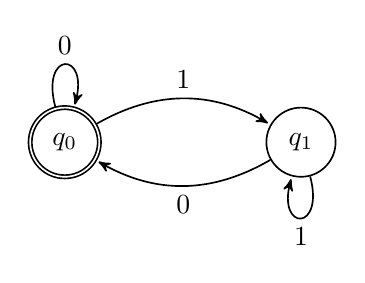
\begin{tikzpicture}[->,>=stealth',shorten >=1pt,auto,node distance=3cm,semithick]
        \tikzstyle{every state}=[fill=white,draw=black,text=black]
      
        \node[state,accepting] (A)                    {$q_0$};
        \node[state]         (B) [right of=A]       {$q_1$};
      
        \path (A) edge [bend left]  node {1} (B)
                  edge [loop above] node {0} (A)
              (B) edge [bend left]  node {0} (A)
                  edge [loop below] node {1} (B);
    \end{tikzpicture}
    \begin{remark}
        \textit{$q_0:$ accepted state}
    \end{remark}
    \textit{$Q = \{q_0,q_1\},\Sigma = \{0,1\},\delta: Q\times \Sigma \rightarrow Q$}
    \begin{table}[htbp]
        \centering
        \begin{tabularx}{\textwidth}{XXXXX}
            \toprule
        $~$ & $0$ & $1$  \\
        \midrule
        $q_0$ & $q_0$ & $q_1$ \\
        $q_1$ & $q_0$ & $q_1$ \\
            \bottomrule
        \end{tabularx}
    \end{table}
\end{example}


\begin{defn}
    \textit{(finite automation)}

    \textit{A \textbf{finite automation} is a 5-tuple ($Q,\Sigma,\delta,q_0,F$), where:}

    \begin{enumerate}
        \item \textit{Q is a finite set called the states}
        \item \textit{$\Sigma$ is the alphabet}
        \item \textit{$\delta:Q\times \Sigma \rightarrow Q$ is the transition function}
        \item \textit{$q_0$ is the start state }
        \item \textit{$F\subseteq Q$ is the set of accept states}
    \end{enumerate}
\end{defn}

\begin{defn}
    \textit{Let $M = (Q,\Sigma,\delta,q_0,F)$ be a finite automation, let w = $w_1w_2\cdots w_n$ be a string, where each $w_i \in \Sigma$.}

    \textit{Then M accept w if there is a sequence of states $r_0,r_1,\cdots,r_n\in Q,$ such that:}

    \begin{enumerate}
        \item $r_0=q_0$
        \item \textit{$\delta(r_i,w_{i+1}) = r_{i+1}$, for $i = 0,1,2,\cdots,n-1$}
        \item $r_n \in F$
    \end{enumerate}
\end{defn}

\begin{defn}
    \textit{If L is the set of strings that M accepts, we say L is the language of M, and write L(M) = L, we say M recognizes/decides/accepts L.}

    \textit{If M accepts no string, it recognizes one language namely, the empty language.}
\end{defn}

\begin{example}
    \textit{L = $\{w\in \{0,1\}^*|w = w_1w_2\cdots w_n,w_n = w_1\}$\\}
    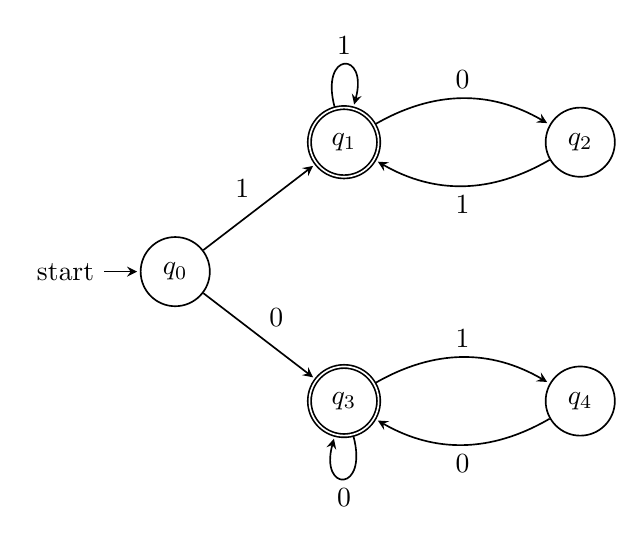
\begin{tikzpicture}[->,>=stealth,shorten >=1pt,auto,node distance=3cm,semithick]
        \tikzstyle{every state}=[fill=white,draw=black,text=black]
      
        \node[state,initial] (A)                    {$q_0$};
        \node[state,accepting]         (B) [above right = 1cm and 1.5cm of A]       {$q_1$};
        \node[state,accepting]         (C) [below right = 1cm and 1.5cm of A] {$q_3$};
        \node[state]         (D) [right of=B]       {$q_2$};
        \node[state]         (E) [right of=C]       {$q_4$};

        \path (A) edge  node {1} (B)
                  edge  node {0} (C)
              (B) edge [loop above] node {1} (B)
                  edge [bend left]  node {0} (D)
              (C) edge [bend left]  node {1} (E)
                  edge [loop below] node {0} (C)
              (D) edge [bend left]  node {1} (B)
              (E) edge [bend left]  node {0} (C);
      \end{tikzpicture}
\end{example}

\subsection{Regular Language}
\begin{defn}
    \textit{(regular language) $L \subseteq \Sigma^*$ is a \textbf{regular language} if there is a finite automation that accepts L}

    \textit{Let $A,B\subseteq\Sigma^*$, define:}

    \begin{itemize}
        \item \textit{(union) $A\cup B = \{x\in \Sigma^*|x\in A$ or $x\in B\}$}
        \item \textit{(concatenation) AB = $\{xy|x\in A,y\in B\}$}
        \item \textit{(star) $A^* = \{x_1x_2\cdots x_k| k\geq 0,x_1,x_2,\cdots,x_k\in A\}$}
    \end{itemize}
\end{defn}

\begin{thm}
    \textit{If $A_1,A_2$ are regular languages, so is $A_1\cup A_2$}

    \begin{proof}
        \textit{Let $M_1 = (Q_1,\Sigma_1,\delta_1,q_{10},F_1)$ accepts $A_1$, $M_2 = (Q_2,\Sigma_2,\delta_2,q_{20},F_2)$ accepts $A_2$, construct M = $(Q,\Sigma,\delta,q_0,F)$:}
        \begin{enumerate}
            \item $Q = Q_1\times Q_2 = \{(r_1,r_2)|r_1\in Q_1,r_2\in Q_2\}$
            \item \textit{$\delta:Q\times \Sigma \rightarrow Q$ is defined as for each $(r_1,r_2)\in Q$, and each $a \in \Sigma$, let $\delta ((r_1,r_2),a) = (\delta_1(r_1,a),\delta_2(r_2,a))$}
            \item $q_0 = (q_{10},q_{20})$
            \item \textit{$F = \{(r_1,r_2)|r_1\in F_1$ or $r_2\in F_2\}$}
        \end{enumerate}
    \end{proof}
    \begin{remark}
        \textit{so is $A\cap B$}
    \end{remark}
\end{thm}

\begin{thm}
    \textit{If $A_1,A_2$ are regular languages, so is $A_1A_2$}

    \begin{itemize}
        \item \textit{\textbf{DFA}: deterministic finite automation}
        \item \textit{\textbf{NFA}: nondeterministic\dots}
    \end{itemize}
    
    \textcolor{red}{\textbf{\textit{If at least one of these processes accepts, then the entire computation accepts.}}}
    \begin{example}
        \textit{NFA:\\}
        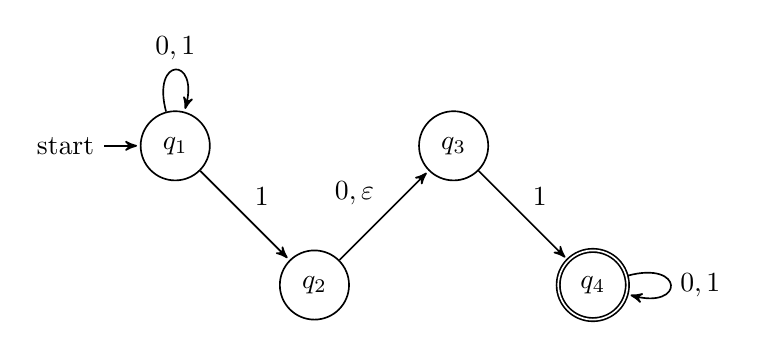
\begin{tikzpicture}[->,>=stealth',shorten >=1pt,auto,node distance=2.5cm,semithick]
            \tikzstyle{every state}=[fill=white,draw=black,text=black]
          
            \node[state,initial] (A)                    {$q_1$};
            \node[state]         (B) [below right of=A]       {$q_2$};
            \node[state]         (C) [above right of=B]       {$q_3$};
            \node[state,accepting]         (D) [below right of=C] {$q_4$};

          
            \path (A) edge              node {1} (B)
                      edge [loop above] node {$0,1$} (A)
                  (B) edge              node {$0,\eps$} (C)
                  (C) edge              node {1} (D)
                  (D) edge [loop right] node {$0,1$} (D);
        \end{tikzpicture}

        \textit{input: $010110$\\}
        \begin{figure}[htbp]
            \centering 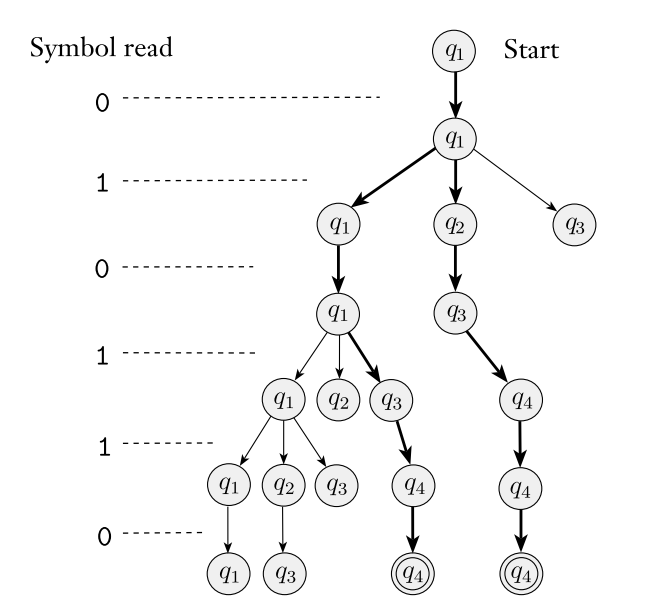
\includegraphics[scale = 0.3]{2.1.png}
            \caption{\textit{The computation of NFA on input 010110}}
        \end{figure}

        \begin{figure}
            \centering 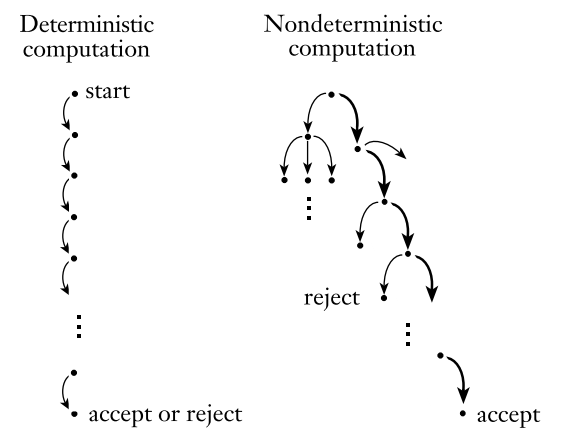
\includegraphics[scale = 0.8]{2.2.png}
            \caption{\textit{Deterministic and nondeterministic computations with an accepting branch}}
        \end{figure}
          
    \end{example}
\end{thm}

\begin{example}
    \textit{Let A be the language consisting of all strings over $\{0,1\}$ containing a $1$ in the third position from the end (e.g., $000100$ is in A but $0011$ is not). The following four-state NFA recognizes A.\\}
    
    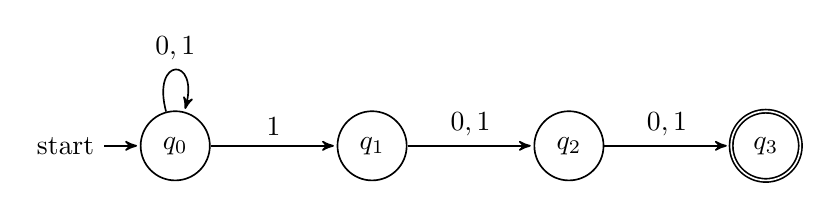
\begin{tikzpicture}[->,>=stealth',shorten >=1pt,auto,node distance=2.5cm,semithick]
        \tikzstyle{every state}=[fill=white,draw=black,text=black]
    
        \node[state,initial] (A)                    {$q_0$};
        \node[state]         (B) [right of=A]       {$q_1$};
        \node[state]         (C) [right of=B]       {$q_2$};
        \node[state,accepting]         (D) [right of=C]       {$q_3$};
    
        \path (A) edge              node {1} (B)
                edge [loop above]   node {$0,1$} (A)
              (B) edge              node {$0,1$} (C)
              (C) edge              node {$0,1$} (D);
    \end{tikzpicture}
\end{example}

\begin{example}
    \textit{$L = \{0^k,2|k~or~3|k\}$\\}
    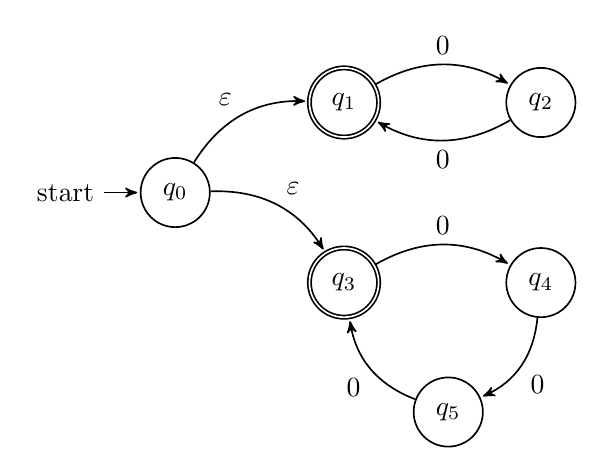
\begin{tikzpicture}[->,>=stealth',shorten >=1pt,auto,node distance=2.5cm,semithick]
        \tikzstyle{every state}=[fill=white,draw=black,text=black]
      
        \node[state,initial] (A)                    {$q_0$};
        \node[state,accepting]         (B) [above right = 0.5cm and 1.5cm of A]       {$q_1$};
        \node[state]         (C) [right of=B]       {$q_2$};
        \node[state,accepting]         (D) [below right = 0.5cm and 1.5cm of A]       {$q_3$};
        \node[state]         (E) [right of=D]       {$q_4$};
        \node[state]         (F) [below right = 1cm and 0.68cm of D]       {$q_5$};
      
        \path (A) edge [bend left]  node {$\eps$} (B)
                  edge [bend left]  node {$\eps$} (D)
              (B) edge [bend left]  node {0} (C)
              (C) edge [bend left]  node {0} (B)
              (D) edge [bend left]  node {0} (E)
              (E) edge [bend left]  node {0} (F)
              (F) edge [bend left]  node {0} (D);
      \end{tikzpicture}
\end{example}

\begin{defn}
    \textit{(NFA)}

    \textit{An \textbf{NFA} is a 5-tuple $(Q,\Sigma,\delta,q_0,F)$,where:}

    \begin{enumerate}
        \item \textit{Q is a finite set of states}
        \item \textit{$\Sigma$ is the alphabet}
        \item \textit{$\delta: Q\times(\Sigma\cup\{\eps\})\rightarrow P(Q)$ is the transive funtion}
        \item \textit{$a_0 \in Q$ is the start state}
        \item \textit{$F \subseteq Q$ is the set of accept states}
    \end{enumerate}
\end{defn}

\begin{defn}
    \

    \textit{Let $N = (Q,\Sigma,\delta,q_0,F)$ be an NFA, and let $w\in \Sigma ^*$. Say N accepts w if we can write $w = y_1y_2\cdots y_m$, where $y_i\in \Sigma\cup\{\eps\}$, and there exist $r_0,r_1,\cdots,r_m\in Q$, such that:}

    \begin{enumerate}
        \item $r_0 = q_0$
        \item \textit{$r_{i+1} \in \delta(r_i,y_{i+1})$ for $i = 0,1,\cdots,m-1$}
        \item $r_m\in F$
    \end{enumerate}
\end{defn}

\begin{thm}
    \textit{Every NFA has  an equivalent DFA}

    \begin{proof}
        
    \end{proof}
\end{thm}
\ifx\allfiles\undefined
\end{document}
\fi